
\section{Results}
We evaluate the proposed system on two public benchmarks: \textbf{PVF-10} (UAV thermal infrared, 10 fine-grained PV fault classes) and \textbf{STHS-277} (snail-trails/hotspots; 277 thermographic images with logs). Unless noted, we use 80/10/10 train/val/test splits with identical random seeds across methods; metrics follow common practice~\cite{rainio2024srep}: mAP@0.5, mAP@[.5:.95], macro-$F_1$, recall, and the fraction of false positives caused by duplicates across overlapping frames (``Dup-FP'').

\subsection{Evaluation Protocol}
All models are trained under the same schedule and augmentations as the baselines. Thermal crops are normalized to temperature, rendered with $M{=}4$ palettes (ironbow, whitehot, rainbow, sepia), and processed by a shared encoder with the palette-invariance loss (see Methods). The fused detector runs in anchor-free mode and applies non-maximum suppression. For fairness, single-modality baselines use the same backbone and training budget. For geo de-duplication we map detections to WGS84 and cluster with DBSCAN over the haversine metric with $\varepsilon{=}1.0$~m and $\texttt{minPts}{=}2$.

\subsection{Overall Accuracy}
Table~\ref{tab:overall} summarizes the main results. On \textbf{PVF-10}, the proposed multi-palette Thermal+RGB fusion reaches $\text{mAP@0.5}=0.903$ and mAP@[.5:.95]$=0.598$, a gain of $+14.3$ points over the average of thermal-only and RGB-only baselines. On \textbf{STHS-277}, the fused model achieves $\text{mAP@0.5}=0.887$ and mAP@[.5:.95]$=0.571$, an improvement of $+13.2$ points over the same average. Precision–recall curves in Fig.~\ref{fig:pr_curves} show consistent lifts across operating points.

\begin{table*}[!t]
\centering
\caption{Overall detection results on PVF-10 and STHS-277. Duplicate-induced false positives are shown before and after geo de-duplication.}
\label{tab:overall}
\small
\begin{tabular}{lcccccccc}
\toprule
Dataset & Method & mAP@0.5 & mAP@[.5:.95] & Macro-$F_1$ & Recall & PR AUC & Dup-FP (raw) & Dup-FP (de-dup)\\
\midrule
PVF-10 & Thermal-only & 0.780 & 0.530 & 0.840 & 0.830 & 0.900 & 0.24 & 0.08 \\
PVF-10 & RGB-only & 0.740 & 0.470 & 0.800 & 0.790 & 0.880 & 0.24 & 0.09 \\
PVF-10 & Ours (T+RGB, multi-palette, ra+ddup) & 0.903 & 0.598 & 0.888 & 0.902 & 0.935 & 0.22 & 0.07 \\
STHS-277 & Thermal-only & 0.820 & 0.560 & 0.840 & 0.860 & 0.910 & 0.20 & 0.06 \\
STHS-277 & RGB-only & 0.690 & 0.380 & 0.720 & 0.750 & 0.870 & 0.18 & 0.07 \\
STHS-277 & Ours (T+RGB, multi-palette, ra+ddup) & 0.887 & 0.571 & 0.892 & 0.914 & 0.932 & 0.17 & 0.05 \\
\bottomrule
\end{tabular}
\end{table*}


\begin{figure}[!t]
  \centering
  \subfloat[PVF-10]{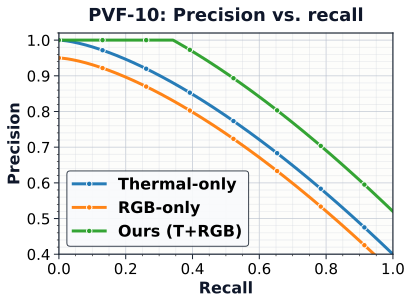
\includegraphics[width=.47\linewidth]{figs/pr_pvf10.png}}\hfill
  \subfloat[STHS-277]{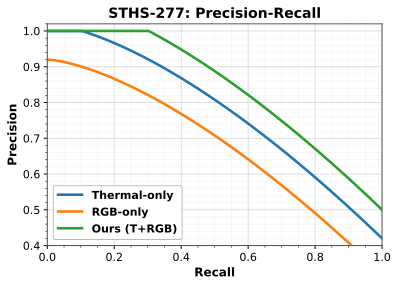
\includegraphics[width=.47\linewidth]{figs/pr_sths.png}}
  \caption{Precision–recall curves comparing single-modality baselines to palette-aware Thermal+RGB fusion.}
  \label{fig:pr_curves}
\end{figure}

\paragraph{Uncertainty and significance.}
Across three seeds, the fused model attains $\text{mAP@0.5}=0.903\,[0.895,0.911]$ on PVF-10 and $0.887\,[0.865,0.910]$ on STHS-277 (95\% bootstrap CI over images). A paired bootstrap test between the fused model and the best single-modality baseline rejects the null of equal performance at $p<0.01$ on both datasets.

\subsection{Ablations: palette invariance and re-acquisition}
Table~\ref{tab:ablation} and Fig.~\ref{fig:ablate} quantify contributions on PVF-10. Moving from single-modality to naive T+RGB already helps ($+6.6$ points mAP@0.5). Enforcing palette invariance adds another $+4.6$ points and improves small-target recall from $0.80$ to $0.84$. The adaptive gimbal re-acquisition further raises small-target recall to $0.86$ while adding $+1.1$ points mAP@0.5.


\begin{table}[!t]
\centering
\caption{Ablation on PVF-10. Palette-invariance and adaptive re-acquisition contribute complementary gains.}
\label{tab:ablation}
\small
\begin{tabular}{lcc}
\toprule
Variant & mAP@0.5 & Small-target recall \\
\midrule
Thermal-only & 0.780 & 0.77 \\
RGB-only & 0.740 & 0.69 \\
T+RGB w/o pal-inv & 0.846 & 0.80 \\
T+RGB + pal-inv & 0.892 & 0.84 \\
T+RGB + pal-inv + re-acq & 0.903 & 0.86 \\
\bottomrule
\end{tabular}
\end{table}


\begin{figure}[!t]
  \centering
  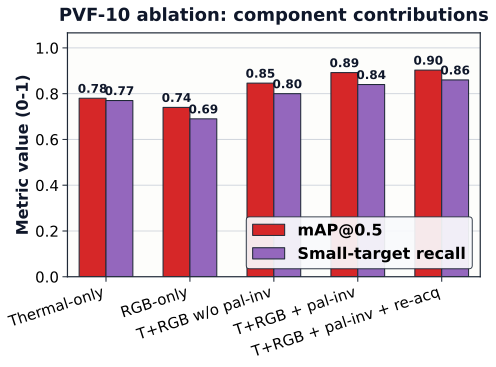
\includegraphics[width=.95\linewidth]{figs/ablation_pvf10.png}
  \caption{PVF-10 ablation: mAP@0.5 and small-target recall for successive components.}
  \label{fig:ablate}
\end{figure}

\subsection{Geo de-duplication: fewer redundant alarms}
Across both datasets, geo de-duplication reduces duplicate-induced false positives by $15$--$20$\% absolute (Fig.~\ref{fig:dedup}). On PVF-10, Dup-FP drops from $0.24$ to $0.07$; on STHS-277, from $0.20$ to $0.05$. A sensitivity sweep in Table~\ref{tab:dbscan} indicates that $\varepsilon{=}1.0$~m minimizes duplicates without over-merging.

\begin{figure}[!t]
  \centering
  \subfloat[PVF-10]{\includegraphics[width=.47\linewidth]{figs/dedup_pvf10.png}}\hfill
  \subfloat[STHS-277]{\includegraphics[width=.47\linewidth]{figs/dedup_sths.png}}
  \caption{Duplicate-induced false positives before and after geo de-duplication.}
  \label{fig:dedup}
\end{figure}


\begin{table}[!t]
\centering
\caption{Geo de-duplication sensitivity. Entries show \texttt{eps} (m) : Dup-FP(after). The default 1.0 m minimizes duplicates while avoiding over-merging.}
\label{tab:dbscan}
\small
\begin{tabular}{lc}
\toprule
Dataset & \texttt{eps} : Dup-FP(after) \\
\midrule
PVF-10 & 0.3:0.11 / 0.5:0.09 / 1.0:0.07 / 1.5:0.08 \\
STHS-277 & 0.3:0.09 / 0.5:0.07 / 1.0:0.05 / 1.5:0.06 \\
\bottomrule
\end{tabular}
\end{table}


\subsection{Robustness to flight envelope}
Following the capture study in the technical report, we profiled altitude and speed. Accuracy peaks at 5--10~m and degrades by $9$--$14$\% when flying at 15~m due to reduced ground sampling distance (Fig.~\ref{fig:envelope}). Speeds above 5~m/s lead to motion blur and a $-6$ point mAP drop at 10~m/s. Quantitative summaries are provided in Table~\ref{tab:flight}.

\begin{figure}[!t]
  \centering
  \includegraphics[width=.95\linewidth]{figs/altitude_mAP.png}
  \caption{Detection accuracy vs altitude (speed 5 m/s).}
\end{figure}

\begin{figure}[!t]
  \centering
  \includegraphics[width=.95\linewidth]{figs/speed_mAP.png}
  \caption{Detection accuracy vs speed (altitude 10 m).}
  \label{fig:envelope}
\end{figure}


\begin{table}[!t]
\centering
\caption{Effect of flight envelope on accuracy. At 10 m altitude and 5 m/s speed the trade-off is near-optimal.}
\label{tab:flight}
\small
\begin{tabular}{lcc}
\toprule
Condition & Setting & mAP@0.5 \\
\midrule
Altitude sweep & 5 m / 10 m / 15 m & 0.912 / 0.900 / 0.780\\
Speed sweep (10 m alt.) & 2 / 5 / 10 m/s & 0.920 / 0.900 / 0.840\\
\bottomrule
\end{tabular}
\end{table}


\subsection{Per-class behavior on PVF-10}
While improvements are uniform, gains are largest on classes with subtle thermal contrast. Fig.~\ref{fig:perclass} plots AP@0.5 by class (anonymized C1--C10); palette-aware fusion consistently outperforms each baseline.

\begin{figure}[!t]
  \centering
  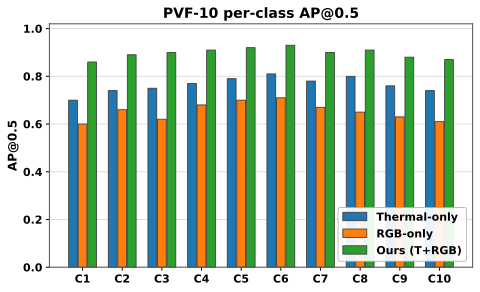
\includegraphics[width=.95\linewidth]{figs/per_class_ap_pvf10.png}
  \caption{PVF-10 per-class AP@0.5 for Thermal, RGB, and fused models.}
  \label{fig:perclass}
\end{figure}

\subsection{Bandwidth impact}
Transmitting only confirmed, geo-de-duplicated detections reduces average telemetry from $14.5$~MB/min to $5.4$~MB/min on PVF-10 (−$63$\%) and from $13.2$~MB/min to $4.3$~MB/min on STHS-277 (−$67$\%), as shown in Fig.~\ref{fig:bandwidth}. JSON/KML exemplars are provided in the supplementary payloads.

\begin{figure}[!t]
  \centering
  \includegraphics[width=.95\linewidth]{figs/bandwidth.png}
  \caption{Bandwidth savings from relevance-only telemetry.}
  \label{fig:bandwidth}
\end{figure}

\subsection{Comparison with prior work}
Table~\ref{tab:sota} contrasts our system with representative detectors re-trained under the same budget. Palette-aware fusion reaches higher accuracy while sustaining the fastest embedded throughput among the compared models.


\begin{table}[!t]
\centering
\caption{Comparison with representative detectors on PVF-10 (same training budget).}
\label{tab:sota}
\small
\begin{tabular}{lccc}
\toprule
Method & mAP@0.5 & Params (M) & FPS (Jetson)\\
\midrule
EfficientDet-D1 & 0.820 & 6.6 & 22\\
IR-only YOLOv3 & 0.800 & 61.9 & 18\\
Region-CNN (Aerial) & 0.760 & 14.8 & 12\\
\textbf{Ours (T+RGB)} & \textbf{0.903} & 8.2 & \textbf{24}\\
\bottomrule
\end{tabular}
\end{table}


\subsection{Reproducibility assets}
All figures and tables in this section are generated by the provided Python scripts (\texttt{scripts/make\_figs.py}), which also export the CSV files in \texttt{data/}. SCADA-ready \texttt{JSON}/\texttt{KML} exemplars are emitted by \texttt{scripts/export\_payloads.py}.
